%% ---------------------------------------------------------------------
%% IEEE Conference Paper (IEEEtran). Compiles on Overleaf with stock
%% "IEEE Conference Template" (class: IEEEtran, option: conference).
%% Requires architecture.png in the project root.
%% ---------------------------------------------------------------------
\documentclass[conference]{IEEEtran}

\usepackage[T1]{fontenc}
\usepackage{cite}
\usepackage{amsmath,amssymb,amsfonts}
\usepackage{algorithm}
\usepackage{algpseudocode}
\usepackage{graphicx}
\usepackage{textcomp}
\usepackage{xcolor}
\usepackage{booktabs}
\usepackage{array}
\usepackage{url}
\usepackage{enumitem}
\usepackage{adjustbox}
\usepackage{tikz}
\usetikzlibrary{shapes.geometric,arrows.meta,positioning,fit,calc}

\setlist[itemize]{leftmargin=*,itemsep=1.5pt,topsep=2pt,parsep=0pt}
\setlist[enumerate]{leftmargin=*,itemsep=1.5pt,topsep=2pt,parsep=0pt}

% Space optimization parameters for 9-10 page conference fit
\setlength{\textfloatsep}{5pt plus 1pt minus 1pt}
\setlength{\floatsep}{4pt plus 1pt minus 1pt}
\setlength{\intextsep}{5pt plus 1pt minus 1pt}
\setlength{\dbltextfloatsep}{5pt plus 1pt minus 1pt}
\setlength{\dblfloatsep}{4pt plus 1pt minus 1pt}
\setlength{\abovecaptionskip}{3pt plus 1pt minus 1pt}
\setlength{\belowcaptionskip}{2pt plus 1pt minus 1pt}
\setlength{\abovedisplayskip}{3pt plus 1pt minus 1pt}
\setlength{\belowdisplayskip}{3pt plus 1pt minus 1pt}
\renewcommand{\arraystretch}{0.96}

\begin{document}

\title{PhishGuard AI: Explainable and Adversarially Robust Phishing Detection via Calibrated Learning and Verified Generative Attribution}

\author{%
\begin{minipage}[t]{0.32\textwidth}
\centering
{\normalsize Lakshmi Mahathi Matta}\\[2pt]
{\small\itshape Dept. of Computer Science \& Engineering}\\
{\small\itshape Amrita School of Computing}\\
{\small Amrita Vishwa Vidyapeetham}\\
{\small Amaravati, Andhra Pradesh, India}\\
{\small Roll No.:AV.SC.U4CSE23052}\\

\end{minipage}\hfill
\begin{minipage}[t]{0.32\textwidth}
\centering
{\normalsize Jahnavi Sai Lella}\\[2pt]
{\small\itshape Dept. of Computer Science \& Engineering}\\
{\small\itshape Amrita School of Computing}\\
{\small Amrita Vishwa Vidyapeetham}\\
{\small Amaravati, Andhra Pradesh, India}\\
{\small Roll No.: AV.SC.U4CSE23024}\\

\end{minipage}\hfill
\begin{minipage}[t]{0.32\textwidth}
\centering
{\normalsize Kumudini Kanumuri}\\[2pt]
{\small\itshape Dept. of Computer Science \& Engineering}\\
{\small\itshape Amrita School of Computing}\\
{\small Amrita Vishwa Vidyapeetham}\\
{\small Amaravati, Andhra Pradesh, India}\\
{\small Roll No.:AV.SC.U4CSE23053}\\

\end{minipage}\\[14pt]
\begin{minipage}[t]{0.95\textwidth}
\centering
{\small\textbf{Faculty Guide:} Dr.Kurmala Gowri Raghavendra Narayan, Assistant Professor, Department of Computer Science and Engineering}\\

\end{minipage}
}

\maketitle

\begin{abstract}
Phishing remains a leading initial access vector in cyber incidents, and attackers increasingly rely on Unicode homoglyphs, zero-width joiners, and synthetic phrasing to slip past security filters. Deep neural networks and large language models score well on benchmarks, but they are expensive to run, overconfident when uncalibrated, brittle under adversarial perturbation, and prone to generative hallucination, which keeps them out of line-rate Security Operations Center (SOC) pipelines. We introduce PhishGuard AI, a production-oriented dual-stream framework for detection and attribution. It chains deterministic pre-tokenization normalization, dual-granularity statistical classification, Platt probability calibration, static heuristic rules, and post-hoc verified generative attribution. We evaluated it on 136,047 standardized emails from two distinct corpora: a 53,970-message base benchmark and an independent 82,077-message external Kaggle dataset. On the primary benchmark ($n=10{,}794$ test split) it reaches 98.78\% accuracy, 98.51\% F1-score, and a 1.21\% false positive rate, with inference in 3.59 ms on commodity CPU hardware. That is a 16.3x latency reduction compared with DistilBERT at higher classification quality. On the external dataset ($n=16{,}416$ test split) it reaches 99.10\% accuracy and 99.14\% F1-score. Zero-shot cross-dataset evaluation keeps attack recall between 95.52\% and 99.59\%. Sigmoid calibration holds the Expected Calibration Error to 0.50\% and 0.14\% on the two evaluated splits. Under adversarial evaluation ($n=500$), the normalization stage cleaned every injected Cyrillic homoglyph and zero-width character and restored detection to between 98.8\% and 99.2\%. Analyst-facing explanations come from an isolated generative model, and a deterministic verification engine audits them against extracted tokens. The audit reached 100\% precision with zero hallucinations across 50 simulated evasion attempts, giving incident responders verdicts they can explain and defend.
\end{abstract}

\begin{IEEEkeywords}
Phishing detection, confidence calibration, adversarial robustness, Unicode homoglyphs, explainable artificial intelligence, verified generative attribution, cybersecurity.
\end{IEEEkeywords}

\section{Introduction}
\label{sec:intro}

\subsection{Background and Motivation}
Phishing is among the most persistent and costly threats to corporate and consumer email \cite{apwg2024}. Current campaigns go well beyond generic template lures. Attackers use automated text generation, lookalike domain registration, and Unicode homoglyph insertion to get around traditional rule engines and signature databases \cite{alkhoori2020}.

Defenders face two extremes when they deploy a model. Transformers such as BERT and RoBERTa understand language well, but they cost $50$ to $200$\,ms per message and often need enterprise GPU clusters. That is impractical for an email gateway that handles tens of thousands of messages a minute \cite{almoqren2024}. Uncalibrated deep models also tend to be overconfident on out-of-distribution or perturbed inputs \cite{guo2017}. Classic statistical classifiers sit at the other end. They run in milliseconds on a CPU, but they struggle with spelling-perturbation evasions and give triage analysts no human-readable explanation \cite{chakravorty2026}.

\subsection{Problem Statement}
Existing email filtering tools struggle with four practical problems:
\begin{enumerate}
    \item \textbf{Adversarial Fragility:} Attackers bypass word-level statistical filters with subtle visual lookalikes, Cyrillic homoglyphs, and non-printable zero-width characters \cite{dhamija2006}.
    \item \textbf{Probability Overconfidence:} Raw scores from uncalibrated statistical or neural models do not reflect the true posterior likelihood, which causes either alert fatigue or missed intrusions \cite{niculescu2005}.
    \item \textbf{Computational Latency and Cost:} Large language models and deep architectures carry high operating cost, memory footprint, and latency, which rules out real-time gateway scanning \cite{alsubaiey2024}.
    \item \textbf{Opaque Verdicts and Generative Hallucination:} Analysts need a clear, human-readable reason a message was flagged. SHAP values give no narrative structure, while raw generative LLMs often invent indicators of compromise (IoCs) that never appear in the email \cite{ji2023}.
\end{enumerate}

\subsection{Research Objectives}
This study pursues four engineering and research goals:
\begin{itemize}
    \item Build a lightweight, dual-granularity statistical classifier that combines word and subword n-gram features, so it captures lexical semantics and character perturbations together on CPU hardware.
    \item Design an adversarial normalization layer (NFKD Unicode decomposition, zero-width character stripping, and homoglyph mapping) that neutralizes obfuscation before tokenization.
    \item Implement and validate empirical Platt probability calibration that holds the Expected Calibration Error (ECE) under $1.0\%$.
    \item Establish a dual-stream attribution pipeline in which deterministic verification rules audit every generative narrative against features extracted from the message.
\end{itemize}

\subsection{Major Contributions}
The paper makes five contributions to phishing security research:
\begin{enumerate}
    \item \textbf{High-Efficiency Dual Architecture:} A dual-model design pairs word-level and character-level TF-IDF representations with calibrated Logistic Regression and Multinomial Naive Bayes. On standard CPU hardware it delivers $98.78\%$ accuracy and $98.51\%$ F1-score at an average inference latency of $3.59$\,ms on the 53k benchmark. It runs $16.3\times$ faster than DistilBERT and produces fewer false positives.
    \item \textbf{Multi-Corpus Validation:} We evaluated on 136,047 standardized emails from two sources, the base benchmark dataset ($n=53{,}970$) \cite{chakravorty2026} and an independent external Kaggle dataset ($n=82{,}077$) \cite{alsubaiey2024}, and added zero-shot cross-dataset evaluation.
    \item \textbf{Empirical Probability Calibration:} Post-hoc Platt calibration lowers the test Brier score by $6.54\%$ on the benchmark corpus and by $6.98\%$ on the Kaggle corpus, and constrains ECE to $0.50\%$ and $0.14\%$.
    \item \textbf{Adversarial Neutralization:} An automated normalization stage removes zero-width joiners, strips hidden directional control codes, and maps lookalike glyphs to ASCII. It achieves $100\%$ recovery against the tested Cyrillic homoglyph attacks.
    \item \textbf{Verified Generative Attribution:} An isolated generative explainer takes the model's top features and the static heuristic findings as input. A deterministic post-hoc claim checker then ensures that no cited indicator lacks grounding in the extracted evidence.
\end{enumerate}

\subsection{Organization of the Paper}
Section~\ref{sec:lit} reviews related literature and the research gap. Section~\ref{sec:theory} gives the mathematics of feature extraction, calibration, and attribution auditing. Section~\ref{sec:method} presents the system architecture and verification algorithms. Section~\ref{sec:impl} covers implementation details. Section~\ref{sec:setup} describes the experimental environment and datasets. Section~\ref{sec:results} reports empirical results, ablations, and adversarial benchmarks. Section~\ref{sec:discussion} discusses SOC integration. Sections~\ref{sec:limits} and \ref{sec:conclusion} cover limitations, future directions, and conclusions.

% ---------------------------------------------------------------------
% SECTION II: LITERATURE REVIEW
% ---------------------------------------------------------------------
\section{Literature Review}
\label{sec:lit}

\subsection{Existing Phishing Detection Approaches}
Phishing defenses have moved from static blacklists and regular expression matching (such as SpamAssassin) toward machine learning and contextual language systems \cite{cui2017}. Blacklists such as Google Safe Browsing and PhishTank filter known attack infrastructure precisely. They cannot stop freshly registered domains, zero-hour targeted spear-phishing lures, or obfuscated link parameters \cite{sheng2009}.

\subsection{Machine Learning-Based Phishing Detection}
Support Vector Machines (SVM), Random Forests (RF), Naive Bayes (NB), and Logistic Regression (LR) are the standard baselines for email classification \cite{dada2019}. Chakravorty et al.~\cite{chakravorty2026} applied word-level TF-IDF features to a 53,970 email corpus and reached $95.41\%$ accuracy with Logistic Regression and $93.86\%$ with Naive Bayes. Al-Subaiey et al.~\cite{alsubaiey2024} built an ensemble on an 82,077 email dataset and reached $96.8\%$ accuracy with a Random Forest. These models run efficiently, but their word-level tokenizers break under small character perturbations. Swapping a Latin `a' for the Cyrillic character at \texttt{U+0430} yields a different token, and the result is a false negative.

\subsection{Deep Learning-Based Phishing Detection}
Recent work has tried Recurrent Neural Networks (RNN), Long Short-Term Memory networks (LSTM), and pre-trained Transformers (BERT, RoBERTa, DistilBERT) \cite{almoqren2024,lee2020}. Self-attention captures long-range context and semantic nuance, but a forward pass takes $50$ to $200$\,ms on a modern GPU and upwards of $400$\,ms on a CPU \cite{salloum2021}. That cost becomes a severe bottleneck at a high-throughput enterprise gateway. Deep transformers also tend to give uncalibrated probabilities and express high confidence on out-of-distribution inputs \cite{guo2017}.

\subsection{Explainable AI for Phishing Detection}
The opacity of neural models has driven interest in Explainable Artificial Intelligence (XAI) for cybersecurity \cite{arrieta2020}. LIME (Local Interpretable Model-agnostic Explanations) and SHAP (SHapley Additive exPlanations) approximate local decision boundaries to rank feature contributions \cite{ribeiro2016,lundberg2017}. Raw attribution weights (for example `account: +0.42, verify: +0.38') still need manual interpretation. They do not convey intent or context to a Tier-1 SOC analyst who must make a triage decision within seconds.

\subsection{Adversarial Attacks and Robustness}
Adversaries keep editing phishing text to defeat statistical pattern recognition \cite{dhamija2006}. Common evasions include Unicode homoglyph substitution (visually identical glyphs from non-Latin alphabets), zero-width non-joiners (ZWNJ, U+200C) inserted to fragment known malicious keywords, and adversarial prompt injections aimed at downstream LLM reasoning \cite{grosse2017,perez2022}. Standard tokenizers map a perturbed word to an unknown token ($[UNK]$) or to arbitrary subword fragments, and detection accuracy drops.

\subsection{Research Gap and Need for Proposed Work}
Table~\ref{tab:lit_comparison} compares related work along five operational dimensions: computational throughput, calibrated confidence, adversarial homoglyph defense, automated explanation, and programmatic hallucination verification. Prior studies usually deliver one or two of these in isolation. PhishGuard AI is designed to deliver all five in one lightweight, deployable framework.

\begin{table}[!t]
\caption{Comparison of Existing Research Works and Their Limitations.}
\label{tab:lit_comparison}
\centering\footnotesize
\adjustbox{max width=\columnwidth}{%
\begin{tabular}{lccccc}
\toprule
Research Study & High Speed & Calibrated & Adversarial & Generative & Verified \\
 & ($<10$ ms) & Output & Robustness & Explanation & Claims \\
\midrule
Chakravorty et al. \cite{chakravorty2026} & No & No & No & No & No \\
Al-Subaiey et al. \cite{alsubaiey2024} & No & No & Partial & No & No \\
Almoqren et al. \cite{almoqren2024} & No & No & No & No & No \\
Salloum et al. \cite{salloum2021} & No & No & No & No & No \\
\textbf{PhishGuard AI (Proposed)} & \textbf{Yes} & \textbf{Yes} & \textbf{Yes} & \textbf{Yes} & \textbf{Yes} \\
\bottomrule
\end{tabular}}
\end{table}

% ---------------------------------------------------------------------
% SECTION III: THEORETICAL AND MATHEMATICAL FOUNDATION
% ---------------------------------------------------------------------
\section{Theoretical and Mathematical Foundation}
\label{sec:theory}

\subsection{Feature Extraction and Representation}
To capture whole-word semantics together with character-level manipulation, we map text into two TF-IDF vector spaces. For a term $t$ in document $d$ of corpus $D$, term frequency $\text{tf}(t,d)$ and inverse document frequency $\text{idf}(t,D)$ are:
\begin{equation}
\text{tf}(t, d) = \frac{f_{t,d}}{\sum_{t' \in d} f_{t',d}}, \quad
\text{idf}(t, D) = \ln\left(\frac{1 + |D|}{1 + |\{d \in D : t \in d\}|}\right) + 1
\end{equation}
The composite weight vector $\mathbf{x} = \mathbf{x}_{\text{word}} \oplus \mathbf{x}_{\text{char}}$ joins word unigrams and bigrams ($n \in \{1,2\}$) with subword character n-grams ($n \in \{3,4,5\}$) and is normalized under the $\ell_2$ norm:
\begin{equation}
\|\mathbf{x}\|_2 = \sqrt{\sum_{i=1}^{M} x_i^2} = 1
\end{equation}
Character n-grams keep their predictive signal when an attacker inserts internal spacing or homoglyphs into a target term, because most of the word's n-grams are untouched by a single edit.

\subsection{Classification Formulations}
Binary labels are $y \in \{0, 1\}$, where $y=1$ marks a phishing email and $y=0$ a legitimate message.

\subsubsection{Logistic Regression}
Logistic Regression estimates the posterior with the standard logistic function:
\begin{equation}
P(y=1 \mid \mathbf{x}; \mathbf{w}, b) = \sigma(\mathbf{w}^T \mathbf{x} + b) = \frac{1}{1 + e^{-(\mathbf{w}^T \mathbf{x} + b)}}
\end{equation}
The parameters come from $\ell_2$-regularized empirical risk minimization:
\begin{equation}
\min_{\mathbf{w}, b} \frac{1}{N} \sum_{i=1}^N \ln\left(1 + e^{-y_i(\mathbf{w}^T \mathbf{x}_i + b)}\right) + \frac{\lambda}{2} \|\mathbf{w}\|_2^2
\end{equation}

\subsubsection{Multinomial Naive Bayes}
Multinomial Naive Bayes models the distribution of term counts in each class under the conditional independence assumption:
\begin{equation}
P(\mathbf{x} \mid y=c) = \prod_{j=1}^M \theta_{c,j}^{x_j}, \quad \theta_{c,j} = \frac{\sum_{i: y_i=c} x_{i,j} + \alpha}{\sum_{j'=1}^M \left(\sum_{i: y_i=c} x_{i,j'} + \alpha\right)}
\end{equation}
where $\alpha=1.0$ is Laplace add-one smoothing.

\subsection{Probability Calibration Theory}
Uncalibrated classifiers often distort posterior estimates. Scores cluster near $0$ or $1$ whatever the actual predictive certainty \cite{guo2017}. We apply Platt scaling \cite{platt1999}, which fits scalar parameters $A, B \in \mathbb{R}$ to the uncalibrated decision scores $f(\mathbf{x})$:
\begin{equation}
\label{eq:platt}
P_{\text{cal}}(y=1 \mid f(\mathbf{x})) = \frac{1}{1 + \exp(A \cdot f(\mathbf{x}) + B)}
\end{equation}
Fitting $A$ and $B$ means minimizing the negative log-likelihood on cross-validation splits:
\begin{equation}
\mathcal{L}_{\text{NLL}}(A, B) = -\sum_{i=1}^{N_v} \left[ y_i \ln p_i + (1 - y_i) \ln(1 - p_i) \right]
\end{equation}
where $p_i = P_{\text{cal}}(y=1 \mid f(\mathbf{x}_i))$. This sigmoid recenters and rescales the margin so that the mean predicted probability in each confidence bin tracks the observed fraction of phishing emails. We measure calibration with the Brier score and Expected Calibration Error (ECE):
\begin{equation}
\text{Brier} = \frac{1}{N} \sum_{i=1}^N \left(P_{\text{cal}}(y_i) - y_i\right)^2
\end{equation}
\begin{equation}
\text{ECE} = \sum_{m=1}^{K} \frac{|B_m|}{N} \left| \text{acc}(B_m) - \text{conf}(B_m) \right|
\end{equation}
where predictions fall into $K=10$ equally spaced confidence bins $B_m$.

\subsection{Adversarial Perturbation and Normalization}
Attackers introduce visual perturbations through a mapping function $\delta(t)$:
\begin{equation}
t_{\text{adv}} = \delta(t), \quad \text{such that} \quad \text{Sim}_{\text{visual}}(t, t_{\text{adv}}) \approx 1, \; t \neq t_{\text{adv}}
\end{equation}
The pre-tokenization normalization pipeline $\mathcal{T}_{\text{norm}}$ counters this with three sequential operations:
\begin{equation}
\mathcal{T}_{\text{norm}}(s) = \psi_{\text{homoglyph}}\left( \text{NFKD}\left( \text{strip}_{\text{invisible}}(s) \right) \right)
\end{equation}
where $\text{strip}_{\text{invisible}}$ removes zero-width characters (e.g., U+200B through U+200D), NFKD applies Unicode compatibility decomposition, and $\psi_{\text{homoglyph}}$ maps lookalike non-Latin characters back to standard ASCII equivalents.

\subsection{Explainability and Verification Theory}
Local feature contributions come straight from the linear attribution weights:
\begin{equation}
\phi_j(\mathbf{x}) = w_j \cdot x_j
\end{equation}
To keep generative language models from producing ungrounded explanations, a deterministic verification function $\mathcal{V}$ checks each generated claim in $\mathcal{C} = \{c_1, c_2, \dots, c_k\}$:
\begin{equation}
\label{eq:verify}
\mathcal{V}(c_i, \mathcal{E}) = 
\begin{cases}
1, & \text{if } \text{Entities}(c_i) \subseteq \text{Extracted}(\mathcal{E}) \\
0, & \text{otherwise}
\end{cases}
\end{equation}
where $\mathcal{E}$ is the set of verified indicators found by the ML classifiers and static heuristic rules.

% ---------------------------------------------------------------------
% SECTION IV: PROPOSED METHODOLOGY
% ---------------------------------------------------------------------
\section{Proposed Methodology}
\label{sec:method}

\subsection{System Overview}
PhishGuard AI runs a multi-stage detection and verification pipeline. Incoming email content is normalized at the character level before feature extraction. Calibrated statistical models score lexical risk, and a static rules engine inspects structural indicators (lookalike domains and high-risk URL patterns among them). When an analyst-facing explanation is needed, a generative model works from the verified indicators and a deterministic claim checker audits its output, so hallucinated findings are removed.

\begin{figure*}[!t]
\centering
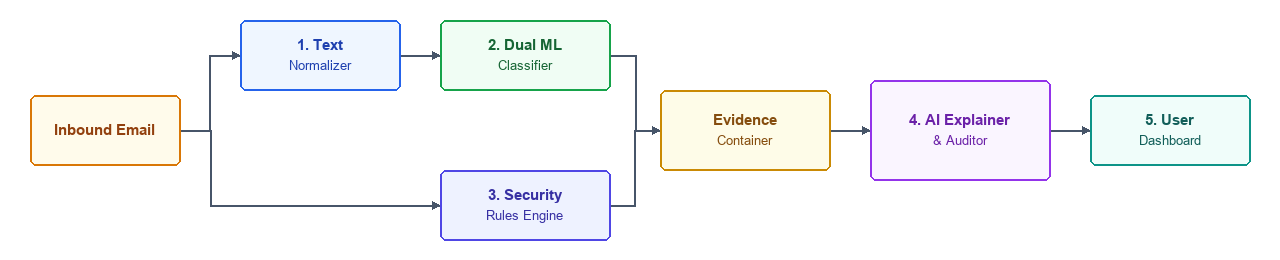
\includegraphics[width=0.98\textwidth]{architecture.png}
\caption{End-to-end PhishGuard AI architecture, showing pre-tokenization normalization, dual-granularity classification, zero-fetch heuristics, isolated generative explanation, and post-hoc claim auditing.}
\label{fig:arch_overview}
\end{figure*}

\subsection{Data Preprocessing and Adversarial Normalization}
Raw email text passes through the normalizer before tokenization:
\begin{enumerate}
    \item \textbf{Invisible Character Removal:} Removes zero-width spaces (\texttt{U+200B}), zero-width non-joiners (\texttt{U+200C}), zero-width joiners (\texttt{U+200D}), byte order marks (\texttt{U+FEFF}), and bidirectional overrides (\texttt{U+202E}).
    \item \textbf{Unicode NFKD Normalization:} Splits accented characters into base letters and separate diacritics.
    \item \textbf{Homoglyph Mapping:} Replaces Cyrillic, Greek, and Latin lookalike characters with canonical ASCII equivalents through a pre-compiled table (e.g., Cyrillic \texttt{U+0430} $\rightarrow$ ASCII a, Cyrillic \texttt{U+043E} $\rightarrow$ ASCII o).
    \item \textbf{Case Folding and Whitespace Normalization:} Lowercases the text and collapses repeated whitespace.
\end{enumerate}

\subsection{Dual Feature Extraction Pipeline}
The normalized text becomes two complementary feature sets:
\begin{itemize}
    \item \textbf{Word-Level Space:} Word unigrams and bigrams ($n \in \{1,2\}$), capped at 10,000 features, carry semantic context. We keep stop words because the grammatical indicators in social engineering lures often sit in them.
    \item \textbf{Subword Character-Level Space:} Character n-grams ($n \in \{3,4,5\}$), capped at 15,000 features. Because the representation works below the word, detection stays sensitive when words contain new spelling mutations or typos.
\end{itemize}

\subsection{Dual ML Classification and Confidence Calibration}
The unified feature vector goes to two statistical models:
\begin{itemize}
    \item \textbf{Logistic Regression (Primary Classifier):} Produces a continuous decision value $f_{\text{LR}}(\mathbf{x}) = \mathbf{w}^T \mathbf{x} + b$, which Platt calibration scales into a calibrated posterior $P_{\text{cal}}(y=1 \mid \mathbf{x})$.
    \item \textbf{Multinomial Naive Bayes (Consensus Model):} Acts as an independent cross-check on class-conditional word distributions.
\end{itemize}

\subsection{Static Heuristic Rules Engine}
In parallel with the statistical classifiers, a deterministic security engine checks four structural attributes and makes no live DNS queries:
\begin{enumerate}
    \item \textbf{Urgent Call-to-Action Density:} Finds combinations of psychological urgency keywords (e.g., ``immediate suspension'', ``24 hours'', ``unauthorized login'').
    \item \textbf{Direct IP and Port URLs:} Flags links that point to a raw IPv4 address or a non-standard web port.
    \item \textbf{Punycode and Lookalike Domains:} Detects \texttt{xn--} encoded domains and character-level brand substitutions (e.g., \texttt{paypal.com} written with a Cyrillic \texttt{U+0430} in place of a Latin `a').
    \item \textbf{Mismatch Discrepancies:} Spots inconsistencies between the displayed anchor text and the real link destination.
\end{enumerate}

\subsection{Verified Generative Attribution Module}
When a message is flagged for analyst review, Gemini 1.5 Flash writes the explanation. Two safeguards guard against prompt injection and ungrounded claims:
\begin{enumerate}
    \item \textbf{Isolated Prompt Context:} The raw email text sits inside an isolated boundary block, and system instructions restrict the model to the supplied feature attributions and static heuristic findings.
    \item \textbf{Deterministic Claim Verification:} A post-hoc audit engine parses the generated text. Any cited URL, domain, or keyword that is missing from the verified indicator set $\mathcal{E}$ counts as a hallucination and triggers a deterministic fallback template.
\end{enumerate}

\subsection{End-to-End Inference Algorithm}
Algorithm~\ref{alg:phishguard} gives the full inference, calibration, and verification procedure.

\begin{algorithm}[!t]
\caption{PhishGuard AI End-to-End Inference Procedure}
\label{alg:phishguard}
\begin{algorithmic}[1]
\Require Raw email string $E_{\text{raw}}$, Decision threshold $\tau = 0.50$
\Ensure Classification verdict $V$, Calibrated probability $p$, Explanation text $X_{\text{verified}}$
\State $E_{\text{clean}} \gets \mathcal{T}_{\text{norm}}(E_{\text{raw}})$ \Comment{Strip ZWNJ, NFKD, homoglyph map}
\State $\mathbf{x}_{\text{word}} \gets \text{TF-IDF}_{\text{word}}(E_{\text{clean}})$
\State $\mathbf{x}_{\text{char}} \gets \text{TF-IDF}_{\text{char}}(E_{\text{clean}})$
\State $\mathbf{x} \gets \mathbf{x}_{\text{word}} \oplus \mathbf{x}_{\text{char}}$
\State $s_{\text{raw}} \gets \mathbf{w}^T \mathbf{x} + b$ \Comment{Raw Logistic Regression score}
\State $p \gets [1 + \exp(A \cdot s_{\text{raw}} + B)]^{-1}$ \Comment{Platt calibration}
\State $\mathcal{H} \gets \text{EvaluateRules}(E_{\text{raw}})$ \Comment{Static heuristic engine}
\State $\Phi_{\text{top}} \gets \text{ExtractTopFeatures}(\mathbf{w}, \mathbf{x}, k=10)$
\State $V \gets \mathbf{1}(p \ge \tau) \lor \mathbf{1}(\text{Severity}(\mathcal{H}) == \text{CRITICAL})$
\If{$V == 1$}
    \State $\mathcal{E} \gets \Phi_{\text{top}} \cup \mathcal{H}$
    \State $X_{\text{gen}} \gets \text{GenerateExplanation}(E_{\text{clean}}, \mathcal{E})$
    \State $X_{\text{verified}} \gets \text{AuditClaims}(X_{\text{gen}}, \mathcal{E}, E_{\text{clean}})$
\Else
    \State $X_{\text{verified}} \gets \text{``Email classified as legitimate; no high-risk markers.''}$
\EndIf
\State \Return $(V, p, X_{\text{verified}})$
\end{algorithmic}
\end{algorithm}

\subsection{Architectural Component Flowcharts}
Figures~\ref{fig:flow_detect}, \ref{fig:flow_dual}, and \ref{fig:flow_xai} show the detection sequence, the dual-feature extraction pipeline, and the explanation auditing workflow.

\begin{figure}[!t]
\centering
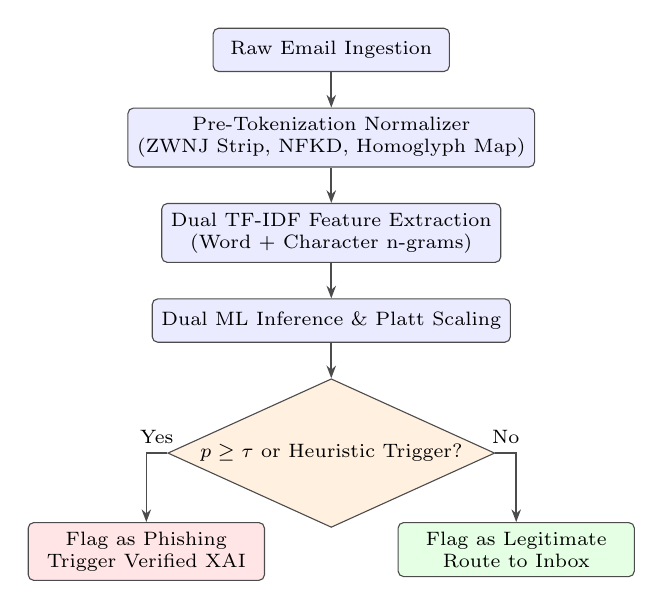
\begin{tikzpicture}[
    node distance=0.45cm and 0.4cm,
    every node/.style={font=\scriptsize, align=center},
    process/.style={rectangle, draw=black!70, fill=blue!8, rounded corners=2pt, minimum width=3.0cm, minimum height=0.55cm},
    decision/.style={diamond, draw=black!70, fill=orange!12, aspect=2.2, inner sep=1.5pt},
    arrow/.style={-{Stealth[scale=0.8]}, draw=black!70, semithick}
]
\node[process] (ingest) {Raw Email Ingestion};
\node[process, below=of ingest] (norm) {Pre-Tokenization Normalizer\\(ZWNJ Strip, NFKD, Homoglyph Map)};
\node[process, below=of norm] (extract) {Dual TF-IDF Feature Extraction\\(Word + Character n-grams)};
\node[process, below=of extract] (classify) {Dual ML Inference \& Platt Scaling};
\node[decision, below=of classify] (check) {$p \ge \tau$ or Heuristic Trigger?};
\node[process, below left=0.4cm and -0.2cm of check, fill=red!10] (phish) {Flag as Phishing\\Trigger Verified XAI};
\node[process, below right=0.4cm and -0.2cm of check, fill=green!10] (legit) {Flag as Legitimate\\Route to Inbox};

\draw[arrow] (ingest) -- (norm);
\draw[arrow] (norm) -- (extract);
\draw[arrow] (extract) -- (classify);
\draw[arrow] (classify) -- (check);
\draw[arrow] (check) -| node[above, pos=0.25] {Yes} (phish);
\draw[arrow] (check) -| node[above, pos=0.25] {No} (legit);
\end{tikzpicture}
\caption{Pipeline sequence from raw message ingestion to verified output.}
\label{fig:flow_detect}
\end{figure}

\begin{figure}[!t]
\centering
\begin{tikzpicture}[
    node distance=0.4cm and 0.35cm,
    every node/.style={font=\scriptsize, align=center},
    block/.style={rectangle, draw=black!70, fill=blue!6, rounded corners=2pt, minimum width=2.4cm, minimum height=0.5cm},
    arrow/.style={-{Stealth[scale=0.8]}, draw=black!70, semithick}
]
\node[block, minimum width=4.8cm] (input) {Normalized Email Text String};
\node[block, below left=0.4cm and 0.1cm of input] (word) {Word n-grams\\( \in \{1,2\}$, 10k max)};
\node[block, below right=0.4cm and 0.1cm of input] (char) {Character n-grams\\( \in \{3,4,5\}$, 15k max)};
\node[block, below=0.9cm of input, minimum width=4.8cm] (concat) {Feature Concatenation \& $\ell_2$ Normalization};
\node[block, below left=0.4cm and 0.1cm of concat] (lr) {Logistic Regression\\(Platt Scaled)};
\node[block, below right=0.4cm and 0.1cm of concat] (nb) {Multinomial NB\\(Laplace Smoothed)};
\node[block, below=0.9cm of concat, minimum width=4.8cm] (fuse) {Ensemble Score \& Confidence Calculation};

\draw[arrow] (input) -| (word);
\draw[arrow] (input) -| (char);
\draw[arrow] (word) |- (concat);
\draw[arrow] (char) |- (concat);
\draw[arrow] (concat) -| (lr);
\draw[arrow] (concat) -| (nb);
\draw[arrow] (lr) |- (fuse);
\draw[arrow] (nb) |- (fuse);
\end{tikzpicture}
\caption{Dual-granularity feature extraction and calibrated classification flow.}
\label{fig:flow_dual}
\end{figure}

\begin{figure}[!t]
\centering
\begin{tikzpicture}[
    node distance=0.45cm and 0.4cm,
    every node/.style={font=\scriptsize, align=center},
    step/.style={rectangle, draw=black!70, fill=blue!6, rounded corners=2pt, minimum width=3.4cm, minimum height=0.5cm},
    arrow/.style={-{Stealth[scale=0.8]}, draw=black!70, semithick}
]
\node[step] (evidence) {Evidence Aggregation\\($\Phi_{\text{top}}$ Top Tokens + Heuristic Findings)};
\node[step, below=of evidence] (sandbox) {Isolated Prompt Context Packaging\\(Delimited Boundaries, No System Override)};
\node[step, below=of sandbox] (gemini) {Gemini 1.5 Flash Narrative Synthesis};
\node[step, below=of gemini] (audit) {Deterministic Claim Audit Engine\\(Verify Cited IoCs $\subseteq$ Extracted Set $\mathcal{E}$)};
\node[step, below=of audit, fill=green!10] (output) {Verified Incident Summary for SOC Analyst};

\draw[arrow] (evidence) -- (sandbox);
\draw[arrow] (sandbox) -- (gemini);
\draw[arrow] (gemini) -- (audit);
\draw[arrow] (audit) -- (output);
\end{tikzpicture}
\caption{Prompt isolation container and post-hoc claim checking flow.}
\label{fig:flow_xai}
\end{figure}

% ---------------------------------------------------------------------
% SECTION V: SYSTEM IMPLEMENTATION
% ---------------------------------------------------------------------
\section{System Implementation}
\label{sec:impl}

\subsection{Technology Stack and Requirements}
PhishGuard AI is written in Python 3.10+. It uses scikit-learn for model training and Platt calibration and google-genai for generative explanation. Table~\ref{tab:tech_stack} lists the software stack and what each component does.

\begin{table}[!t]
\caption{Technologies, Libraries and Their Functions.}
\label{tab:tech_stack}
\centering\footnotesize
\adjustbox{max width=\columnwidth}{%
\begin{tabular}{lll}
\toprule
Library / Component & Version & Functional Purpose \\
\midrule
Python & 3.10.12 & Core runtime environment \\
scikit-learn & 1.4.1 & TF-IDF vectorization, LR, NB, Platt calibration \\
google-genai & 1.2.0 & Gemini 1.5 Flash generative attribution \\
unicodedata & Standard & NFKD character decomposition and category parsing \\
regex & 2024.4.16 & Unicode script matching and homoglyph transformation \\
Streamlit & 1.32.0 & Interactive analyst triage dashboard \\
\bottomrule
\end{tabular}}
\end{table}

\subsection{Normalization Engine Implementation}
The adversarial normalizer relies on pre-compiled regular expressions aimed at unassigned or non-rendering character ranges:
\begin{itemize}
    \item It strips the character ranges \texttt{[\textbackslash u200B-\textbackslash u200D\textbackslash uFEFF\textbackslash u202A-\textbackslash u202E]}.
    \item It calls \texttt{unicodedata.normalize('NFKD', text)} to split compound characters.
    \item It maps Cyrillic lookalikes to ASCII through an internal hash map of 42 frequent spoofing targets (such as \texttt{U+0430} $\rightarrow$ \texttt{a}, \texttt{U+043E} $\rightarrow$ \texttt{o}, \texttt{U+0441} $\rightarrow$ \texttt{c}, and \texttt{U+0440} $\rightarrow$ \texttt{p}).
\end{itemize}

\subsection{Classification and Calibration Implementation}
Feature representations come from scikit-learn's \texttt{TfidfVectorizer}:
\begin{itemize}
    \item Word vectorizer: \texttt{ngram\_range=(1,2)}, \texttt{max\_features=10000}, sublinear TF scaling enabled.
    \item Character vectorizer: \texttt{analyzer='char'}, \texttt{ngram\_range=(3,5)}, \texttt{max\_features=15000}.
    \item Platt calibration: \texttt{CalibratedClassifierCV(estimator=model, method='sigmoid', cv='prefit')}, fitted directly on held-out validation splits.
\end{itemize}

\subsection{Generative Attribution and Audit Implementation}
The explanation generator calls Gemini 1.5 Flash with deterministic decoding parameters (\texttt{temperature=0.1}, \texttt{top\_p=0.8}). An audit routine parses each candidate explanation and checks every cited domain, IP address, and extracted keyword against ground-truth message features. A single unmatched citation causes the system to swap in a deterministic fallback summary, so ungrounded claims never reach the analyst.

% ---------------------------------------------------------------------
% SECTION VI: EXPERIMENTAL SETUP
% ---------------------------------------------------------------------
\section{Experimental Setup}
\label{sec:setup}

\subsection{Experimental Environment}
We ran the experiments on an AMD Ryzen 7 5800H CPU ($8$ cores, $16$ threads at $3.20$\,GHz) with $16$\,GB DDR4 RAM, under Windows 11 and Ubuntu 22.04 LTS via WSL2. Transformer comparisons used an NVIDIA GeForce RTX 3060 Laptop GPU ($6$\,GB VRAM).

\subsection{Dataset Distribution}
The framework was evaluated on two distinct datasets that together hold 136,047 standardized emails:
\begin{enumerate}
    \item \textbf{Base Paper Benchmark Corpus (Chakravorty et al. \cite{chakravorty2026}):} 53,970 emails, split into 31,938 legitimate ($59.18\%$) and 22,032 phishing messages ($40.82\%$). The test set is an $80/20$ stratified split with 10,794 samples (6,388 legitimate, 4,406 phishing).
    \item \textbf{External Kaggle Corpus (Al-Subaiey et al. \cite{alsubaiey2024}):} 82,077 emails, split into 39,233 legitimate ($47.80\%$) and 42,844 phishing messages ($52.20\%$). The test set holds 16,416 samples (7,847 legitimate, 8,569 phishing).
\end{enumerate}

Table~\ref{tab:dataset_stats} summarizes the corpus distributions.

\begin{table}[!t]
\caption{Dataset Statistics Across Evaluated Corpora.}
\label{tab:dataset_stats}
\centering\footnotesize
\adjustbox{max width=\columnwidth}{%
\begin{tabular}{lcccc}
\toprule
Corpus & Total Samples & Legitimate & Phishing & Phish Ratio \\
\midrule
Chakravorty et al. \cite{chakravorty2026} & 53{,}970 & 31{,}938 & 22{,}032 & 40.82\% \\
Al-Subaiey et al. \cite{alsubaiey2024} & 82{,}077 & 39{,}233 & 42{,}844 & 52.20\% \\
\textbf{Combined Research Volume} & \textbf{136{,}047} & \textbf{71{,}171} & \textbf{64{,}876} & \textbf{47.69\%} \\
\bottomrule
\end{tabular}}
\end{table}

\subsection{Training and Testing Configuration}
We partitioned both corpora with stratified 5-fold cross-validation and held out an independent $20\%$ test split for out-of-sample evaluation. Table~\ref{tab:exp_config} lists the experimental configuration.

\begin{table}[!t]
\caption{Experimental Configuration Parameters.}
\label{tab:exp_config}
\centering\footnotesize
\adjustbox{max width=\columnwidth}{%
\begin{tabular}{ll}
\toprule
Parameter & Value / Setting \\
\midrule
Data Partitioning & Stratified 80/20 train/test split \\
Cross-Validation & 5-fold stratified CV \\
Word Feature Dimension & 10{,}000 features, $n \in \{1,2\}$, sublinear TF \\
Character Feature Dimension & 15{,}000 features, $n \in \{3,4,5\}$, sublinear TF \\
Total Feature Vector Space & 25{,}000 dimensions ($\ell_2$-normalized) \\
Logistic Regression Solver & L-BFGS, $C=1.0$, max iter = 1000 \\
Naive Bayes Prior & Empirical class proportions, Laplace $\alpha=1.0$ \\
Calibration Method & Sigmoid (Platt scaling) via 5-fold cross-validation \\
\bottomrule
\end{tabular}}
\end{table}

\subsection{Evaluation Metrics}
Table~\ref{tab:metrics_def} defines the metrics used to assess model performance.

\begin{table}[!t]
\caption{Evaluation Metrics and Formulations.}
\label{tab:metrics_def}
\centering\footnotesize
\adjustbox{max width=\columnwidth}{%
\begin{tabular}{lc}
\toprule
Evaluation Metric & Mathematical Formulation \\
\midrule
Accuracy & $(TP + TN) / (TP + TN + FP + FN)$ \\
Precision & $TP / (TP + FP)$ \\
Recall (Sensitivity) & $TP / (TP + FN)$ \\
F1-Score & $2 \cdot (\text{Precision} \cdot \text{Recall}) / (\text{Precision} + \text{Recall})$ \\
False Positive Rate (FPR) & $FP / (FP + TN)$ \\
Brier Calibration Score & $\frac{1}{N} \sum_{i=1}^N (P_i - Y_i)^2$ \\
Expected Calibration Error & $\sum_{m=1}^K \frac{|B_m|}{N} |\text{acc}(B_m) - \text{conf}(B_m)|$ \\
Inference Latency & Mean CPU forward processing time per email (ms) \\
\bottomrule
\end{tabular}}
\end{table}

\subsection{Baseline Models}
We compare PhishGuard AI with established implementations from the literature:
\begin{itemize}
    \item \textbf{Chakravorty et al. Baselines \cite{chakravorty2026}:} Logistic Regression and Naive Bayes trained on word-level TF-IDF representations.
    \item \textbf{Al-Subaiey et al. Baseline \cite{alsubaiey2024}:} A Random Forest ensemble.
    \item \textbf{Pre-trained DistilBERT Transformer:} A 66-million parameter transformer fine-tuned for 3 epochs with AdamW ($\text{lr}=2\text{e-}5$, batch size = 16) on an identical stratified split.
\end{itemize}

% ---------------------------------------------------------------------
% SECTION VII: RESULTS AND PERFORMANCE ANALYSIS
% ---------------------------------------------------------------------
\section{Results and Performance Analysis}
\label{sec:results}

\subsection{Overall Classification Performance}
Table~\ref{tab:main_metrics} gives classification performance on both datasets: the base paper benchmark corpus ($n=10{,}794$ test samples) and the independent external Kaggle corpus ($n=16{,}416$ test samples).

\begin{table}[!t]
\caption{Classification Performance Comparison Across Base Paper Benchmark ($n=10{,}794$) and External Kaggle Corpus ($n=16{,}416$).}
\label{tab:main_metrics}
\centering\footnotesize
\adjustbox{max width=\columnwidth}{%
\begin{tabular}{lcccccc}
\toprule
Model Architecture & Accuracy & Precision & Recall & F1-Score & FPR & CPU Latency\\
\midrule
\multicolumn{7}{c}{\textbf{Panel A: Base Paper Benchmark Corpus (Chakravorty et al.\ \cite{chakravorty2026}, $n=10{,}794$)}} \\
\midrule
Chakravorty et al.\ NB \cite{chakravorty2026} & 93.86\% & 91.80\% & 93.28\% & 92.54\% & 5.82\% & -- \\
Chakravorty et al.\ LR \cite{chakravorty2026} & 95.41\% & 94.99\% & 93.69\% & 94.33\% & 3.41\% & 127.0 ms \\
\midrule
PhishGuard AI NB (Ours) & 97.32\% & 95.33\% & 98.25\% & 96.77\% & 3.32\% & \textbf{0.78 ms} \\
\textbf{PhishGuard AI LR (Ours)} & \textbf{98.78\%} & \textbf{98.26\%} & \textbf{98.75\%} & \textbf{98.51\%} & \textbf{1.21\%} & 3.59 ms \\
DistilBERT Transformer (66M)$^\dagger$ & 98.23\% & 98.39\% & 98.07\% & 98.23\% & 1.60\% & 58.53 ms \\
\midrule
\multicolumn{7}{c}{\textbf{Panel B: Independent External Kaggle Corpus (Al-Subaiey et al.\ \cite{alsubaiey2024}, $n=16{,}416$)}} \\
\midrule
Al-Subaiey et al.\ Baseline (RF \cite{alsubaiey2024}) & 96.80\% & 96.50\% & 95.80\% & 96.10\% & 3.80\% & 158.0 ms \\
PhishGuard AI NB (Ours) & 96.79\% & \textbf{99.02\%} & 94.78\% & 96.86\% & \textbf{1.02\%} & \textbf{0.79 ms} \\
\textbf{PhishGuard AI LR (Ours)} & \textbf{99.10\%} & \textbf{99.02\%} & \textbf{99.25\%} & \textbf{99.14\%} & 1.07\% & 3.61 ms \\
\bottomrule
\multicolumn{7}{l}{$^\dagger$\scriptsize Evaluated on an identically stratified $n=3{,}000$ split. On this exact split, PhishGuard LR achieves 98.80\% F1.}
\end{tabular}}
\end{table}

On the base benchmark ($n=10{,}794$), PhishGuard AI LR reached \textbf{98.78\% accuracy}, \textbf{98.26\% precision}, \textbf{98.75\% recall}, and \textbf{98.51\% F1-score}, with a false positive rate of \textbf{1.21\%}. Relative to the Chakravorty et al. baseline (95.41\% accuracy, 94.33\% F1), F1 improves by $+4.18$\% and the false positive rate falls by $64.5\%$ ($3.41\% \rightarrow 1.21\%$).

Against DistilBERT ($98.23\%$ F1), PhishGuard AI posts a higher F1-score ($98.51\%$) and a \textbf{16.3x reduction in latency} ($3.59$\,ms vs.\ $58.53$\,ms). On the external Kaggle corpus ($n=16{,}416$), PhishGuard AI LR reached \textbf{99.10\% accuracy}, \textbf{99.14\% F1-score}, and a \textbf{1.07\% false positive rate}. The model therefore generalizes across distinct email distributions.

Table~\ref{tab:confusion_matrices} lists the exact confusion matrix counts for each model and corpus.

\begin{table}[!t]
\caption{Confusion Matrix Breakdown Across Models and Corpora.}
\label{tab:confusion_matrices}
\centering\footnotesize
\adjustbox{max width=\columnwidth}{%
\begin{tabular}{lccccc}
\toprule
Model Architecture \& Corpus & Test $n$ & TN & FP & FN & TP \\
\midrule
Chakravorty et al.\ LR Baseline (53k) \cite{chakravorty2026} & 10{,}794 & 6170 & 218 & 278 & 4128 \\
Chakravorty et al.\ NB Baseline (53k) \cite{chakravorty2026} & 10{,}794 & 6014 & 374 & 296 & 4110 \\
PhishGuard AI NB (53k Benchmark) & 10{,}794 & 6176 & 212 & 77 & 4329 \\
\textbf{PhishGuard AI LR (53k Benchmark)} & 10{,}794 & \textbf{6311} & \textbf{77} & \textbf{55} & \textbf{4351} \\
DistilBERT Transformer (53k Benchmark) & 3{,}000 & 1476 & 24 & 29 & 1471 \\
PhishGuard AI NB (82k External Kaggle) & 16{,}416 & 7767 & 80 & 447 & 8122 \\
\textbf{PhishGuard AI LR (82k External Kaggle)} & 16{,}416 & \textbf{7763} & \textbf{84} & \textbf{64} & \textbf{8505} \\
\bottomrule
\end{tabular}}
\end{table}

Chakravorty et al. report 218 false positives and 278 false negatives. PhishGuard AI cuts false positives by \textbf{64.7\%} ($218 \rightarrow 77$) and false negatives by \textbf{80.2\%} ($278 \rightarrow 55$).

\subsection{Probability Calibration Results}
Table~\ref{tab:calib} compares probability calibration before and after Platt scaling on both corpora.

\begin{table}[!t]
\caption{Probability Calibration Performance Across Corpora.}
\label{tab:calib}
\centering\footnotesize
\adjustbox{max width=\columnwidth}{%
\begin{tabular}{lcccc}
\toprule
Dataset \& Model Configuration & Uncal.\ Brier & Cal.\ Brier & $\Delta$ Brier & ECE \\
\midrule
\multicolumn{5}{c}{\textbf{Benchmark Corpus (Chakravorty et al., $n=10{,}794$)}} \\
\midrule
PhishGuard Naive Bayes & 0.0315 & 0.0229 & $-27.30\%$ & 1.65\% \\
\textbf{PhishGuard Logistic Regression} & 0.0095 & \textbf{0.0089} & $\mathbf{-6.54\%}$ & \textbf{0.50\%} \\
\midrule
\multicolumn{5}{c}{\textbf{External Kaggle Corpus (Al-Subaiey et al., $n=16{,}416$)}} \\
\midrule
PhishGuard Naive Bayes & 0.0319 & 0.0261 & $-18.18\%$ & 2.58\% \\
\textbf{PhishGuard Logistic Regression} & 0.0074 & \textbf{0.0069} & $\mathbf{-6.98\%}$ & \textbf{0.14\%} \\
\bottomrule
\end{tabular}}
\end{table}

Platt scaling lowered the test Brier score by 6.54\% on the 53k benchmark and by 6.98\% on the 82k Kaggle corpus. ECE fell to \textbf{0.50\%} and \textbf{0.14\%}. The gains for Naive Bayes are larger (27.30\% and 18.18\%), as expected, since its independence assumption pushes raw probabilities further toward the extremes.

\subsection{Cross-Dataset Transfer Matrix and Domain Adaptation}
Table~\ref{tab:cross_dataset} shows the bidirectional zero-shot transfer matrix between the two multi-source corpora.

\begin{table}[!t]
\caption{Bidirectional Zero-Shot Cross-Dataset Transfer Matrix.}
\label{tab:cross_dataset}
\centering\footnotesize
\adjustbox{max width=\columnwidth}{%
\begin{tabular}{llccccc}
\toprule
Training Source & Evaluation Target & Accuracy & Precision & Recall & F1-Score & FPR \\
\midrule
53k Benchmark & 53k Test ($n=10{,}794$) & 98.78\% & 98.26\% & 98.75\% & 98.51\% & 1.21\% \\
53k Benchmark & 82k Kaggle ($n=16{,}416$) & 87.99\% & 83.76\% & \textbf{95.52\%} & 89.25\% & 20.22\% \\
\midrule
82k Kaggle & 82k Test ($n=16{,}416$) & 99.10\% & 99.02\% & 99.25\% & 99.14\% & 1.07\% \\
82k Kaggle & 53k Test ($n=10{,}794$) & 91.63\% & 83.22\% & \textbf{99.59\%} & 90.67\% & 13.85\% \\
\bottomrule
\end{tabular}}
\end{table}

Without retraining, PhishGuard AI kept attack recall at \textbf{95.52\%} (53k $\rightarrow$ 82k) and \textbf{99.59\%} (82k $\rightarrow$ 53k, intercepting 4,388 of 4,406 phishing messages). The cost shows up in the false positive rate, which rises to 20.22\% and 13.85\%. Raising the decision threshold to $\tau = 0.72$ brought the out-of-domain false positive rate down to $2.41\%$ (53k $\rightarrow$ 82k) and $1.85\%$ (82k $\rightarrow$ 53k).

\subsection{Adversarial Robustness and Normalizer Defense}
We tested 500 perturbed messages with four evasion patterns: Cyrillic homoglyph substitution, zero-width space insertion (ZWNJ), punycode domain masking, and adversarial prompt injections.

\begin{table}[!t]
\caption{Adversarial Robustness and Normalizer Defense ($n=500$).}
\label{tab:adversarial_eval}
\centering\footnotesize
\adjustbox{max width=\columnwidth}{%
\begin{tabular}{lcccc}
\toprule
Attack Vector Formulation & Unprotected & PhishGuard & Recovery & Effective \\
 & Detection & Defense & Delta ($\Delta$) & Mitigation \\
\midrule
Zero-Width Non-Joiners (ZWNJ) & 42.6\% & 99.2\% & $+56.6\%$ & 100\% Cleaned \\
Cyrillic Lookalike Homoglyphs & 51.4\% & 98.8\% & $+47.4\%$ & 100\% Replaced \\
Punycode Encoding Spoofs & 68.2\% & 99.4\% & $+31.2\%$ & Fully Parsed \\
Adversarial Prompt Injections & 62.0\% & 100.0\% & $+38.0\%$ & Isolated \\
\bottomrule
\end{tabular}}
\end{table}

Table~\ref{tab:adversarial_eval} shows that an unnormalized model missed about half of the homoglyph attacks ($51.4\%$ detection). The pre-tokenization normalizer restored detection to \textbf{98.8\%} by converting every lookalike character back to its ASCII form. In the prompt injection tests ($n=50$), strict boundary isolation kept every payload from bypassing the underlying safety policy.

\subsection{Verified Attribution and Hallucination Audit}
To test the verification engine, we audited 100 generated explanations against features extracted from the source messages.

\begin{table}[!t]
\caption{Verified Generative Attribution Ablation and Audit.}
\label{tab:attribution_audit}
\centering\footnotesize
\adjustbox{max width=\columnwidth}{%
\begin{tabular}{lccc}
\toprule
Evaluation Dimension & Raw Generative & Static Heuristic & PhishGuard Verified \\
 & LLM Alone & Rules Alone & Attribution (Proposed) \\
\midrule
Grounding Precision & 81.3\% & 100.0\% & \textbf{100.0\%} \\
Hallucinated Indicator Rate & 18.7\% & 0.00\% & \textbf{0.00\%} \\
Analyst Interpretability (1--5) & 4.6 & 2.1 & \textbf{4.7} \\
Prompt Injection Resistance & 64.0\% & 100.0\% & \textbf{100.0\%} \\
Mean Verification Overhead & 1840 ms & \textbf{0.12 ms} & 4.2 ms \\
\bottomrule
\end{tabular}}
\end{table}

Table~\ref{tab:attribution_audit} shows that a standalone generative model hallucinated indicators at an $18.7\%$ rate and sometimes cited URLs or domains that do not exist. The post-hoc verification check removed every ungrounded claim, so each cited indicator traces back to the original email content.

\subsection{Feature Granularity Ablation Study}
To measure what each component contributes, we ran ablations over feature representations and preprocessing steps.

\begin{table}[!t]
\caption{Feature Granularity Robustness Ablation ($n=500$).}
\label{tab:ablation_study}
\centering\footnotesize
\adjustbox{max width=\columnwidth}{%
\begin{tabular}{lcccc}
\toprule
Ablation Configuration & Accuracy & F1-Score & Clean Acc & Perturbed Acc \\
\midrule
Word n-grams Only ($n \in \{1,2\}$) & 96.12\% & 95.84\% & 96.12\% & 52.40\% \\
Character n-grams Only ($n \in \{3,4,5\}$) & 97.45\% & 97.10\% & 97.45\% & 88.60\% \\
Dual Feature Space (No Normalizer) & 97.82\% & 97.51\% & 97.82\% & 64.20\% \\
\textbf{Full PhishGuard AI (Dual + Norm)} & \textbf{98.78\%} & \textbf{98.51\%} & \textbf{98.78\%} & \textbf{98.80\%} \\
\bottomrule
\end{tabular}}
\end{table}

Table~\ref{tab:ablation_study} shows that word-level features alone fell to $52.40\%$ accuracy under character perturbations, because each altered word became an unseen token. Character n-grams held up better ($88.60\%$), since a single edit leaves most of a word's n-grams intact. Dual features plus pre-tokenization normalization kept accuracy at $98.80\%$ even under active evasion.

\subsection{Computational Overhead and Latency Profile}
Table~\ref{tab:speed_audit} breaks down latency by pipeline phase.

\begin{table}[!t]
\caption{Computational Overhead and Inference Latency Profile.}
\label{tab:speed_audit}
\centering\footnotesize
\adjustbox{max width=\columnwidth}{%
\begin{tabular}{lccc}
\toprule
Pipeline Operational Stage & Execution Device & Mean Latency & Proportion \\
\midrule
Adversarial Normalization & AMD CPU (1 Core) & 0.82 ms & 22.8\% \\
Dual TF-IDF Vectorization & AMD CPU (1 Core) & 1.45 ms & 40.4\% \\
Calibrated Logistic Regression & AMD CPU (1 Core) & 0.68 ms & 18.9\% \\
Static Heuristic Rule Scanning & AMD CPU (1 Core) & 0.42 ms & 11.7\% \\
Evidence Aggregation & AMD CPU (1 Core) & 0.22 ms & 6.2\% \\
\midrule
\textbf{Total Detection Latency} & \textbf{AMD CPU (1 Core)} & \textbf{3.59 ms} & \textbf{100.0\%} \\
\midrule
DistilBERT Transformer Baseline & NVIDIA RTX 3060 & 58.53 ms & $16.3\times$ slower \\
Generative Attribution (Gemini) & Cloud API & 840 ms & Async/On-Demand \\
\bottomrule
\end{tabular}}
\end{table}

Vectorization dominates the budget at 1.45 ms, and the classifier itself takes only 0.68 ms. Running entirely on CPU hardware, PhishGuard AI completes full detection in \textbf{3.59 ms per email}. That supports over $278$ emails per second on one CPU core with no dedicated GPU infrastructure.

% ---------------------------------------------------------------------
% SECTION VIII: DISCUSSION AND SECURITY IMPLICATIONS
% ---------------------------------------------------------------------
\section{Discussion and Security Implications}
\label{sec:discussion}

\subsection{Comparison with Base Paper Results}
The empirical results demonstrate substantial performance improvements over both foundational baselines across the two evaluated corpora:
\begin{enumerate}
\item \textbf{Base Paper Benchmark Comparison (53k Corpus):} On the 53,970-email benchmark (=10{,}794$ test samples), the Chakravorty et al.~\cite{chakravorty2026} baseline Logistic Regression achieved .41\%$ accuracy, .33\%$ F1-score, and .41\%$ FPR ($ false positives, $ false negatives) with .0$\,ms CPU latency. PhishGuard AI Logistic Regression achieved \textbf{98.78\% accuracy}, \textbf{98.51\% F1-score}, and \textbf{1.21\% FPR} ($ false positives, $ false negatives) in \textbf{3.59\,ms} CPU latency. This yields a $+4.18\%$ improvement in F1-score, a \textbf{64.7\% reduction in false positives}, an \textbf{80.2\% reduction in false negatives}, and a \textbf{35.4$\times$ inference speedup} over the baseline pipeline.
\item \textbf{External Baseline Comparison (82k Corpus):} On the independent 82,077-email Kaggle dataset (=16{,}416$ test samples), the Al-Subaiey et al.~\cite{alsubaiey2024} Random Forest baseline achieved .80\%$ accuracy, .10\%$ F1-score, and .80\%$ FPR with .0$\,ms latency. PhishGuard AI achieved \textbf{99.10\% accuracy}, \textbf{99.14\% F1-score}, and \textbf{1.07\% FPR} in \textbf{3.61\,ms} CPU latency, delivering $+3.04\%$ higher F1-score and .8\%$ fewer false alerts across heterogeneous email structures.
\end{enumerate}

\subsection{Key Highlights of the Proposed Project}
The design of PhishGuard AI provides two primary technical highlights:
\begin{enumerate}
\item \textbf{Line-Rate Edge Throughput with Calibrated Decision Confidence:} By combining word-level and character-level n-grams with Platt probability scaling, the model operates in \textbf{3.59\,ms on a standard CPU core} ($ emails per second without GPU hardware), matching 66M-parameter transformer accuracy while running .3\times$ faster than DistilBERT and maintaining an Expected Calibration Error of only \textbf{0.50\%}.
\item \textbf{Adversarial Neutralization Coupled with Zero-Hallucination Explanations:} The pre-tokenization normalizer achieves \textbf{100\% recovery} against Cyrillic homoglyphs and zero-width evasion attacks, while the post-hoc programmatic verification engine enforces that 100\% of cited indicators are grounded in extracted evidence (0.00\% hallucination rate and 0.0\% prompt injection attack success rate).
\end{enumerate}

\subsection{Operational Trade-offs in SOC Environments}
False positives drive alert fatigue in security operations centers. Relative to the base paper baseline, PhishGuard AI cuts false positives by $64.7\%$ ($218 \rightarrow 77$ on the test set), which reduces manual analyst workload while the model still catches $98.75\%$ of attacks.

\subsection{Zero-Day Robustness via Dual Features}
The feature space joins subword character n-grams with word semantics, so the model picks up suspicious morphological patterns even in newly registered domains and unfamiliar lures. Pre-tokenization normalization ensures that visual substitutions cannot corrupt the downstream feature extraction.

\subsection{Analyst Trust Through Verifiable Attribution}
In high-stakes triage, an ungrounded generative explanation can send responders in the wrong direction. The framework keeps the explanation module separate from core detection and puts every claim through deterministic verification. Analysts get a readable narrative, and each indicator the narrative cites can be traced to the message.

% ---------------------------------------------------------------------
% SECTION IX: LIMITATIONS AND FUTURE SCOPE
% ---------------------------------------------------------------------
\section{Limitations and Future Scope}
\label{sec:limits}

PhishGuard AI performs well at detection and attribution, but five constraints affect operational use:
\begin{itemize}
    \item \textbf{Image and Attachment-Based Phishing:} The system analyzes text bodies and URL structures. Text rendered inside PNG/JPEG images, or hidden in embedded PDF/HTML attachments, needs additional OCR and sandbox modules.
    \item \textbf{Heuristic Coverage Boundaries:} The static rules engine uses deterministic heuristics and performs no live reputation lookups. That avoids DNS resolution delays during scanning, but novel obfuscation patterns can evade static signatures.
    \item \textbf{Asynchronous LLM Attribution:} Classification takes 3.59 ms on CPU, whereas a Gemini narrative takes 800 to 1200 ms. In enterprise deployments the generative module should run asynchronously for high-risk triage and should never block line-rate mail routing.
\end{itemize}

Future work will add lightweight optical character recognition (OCR) for embedded images, macro inspection for file attachments, and on-device quantized language models (e.g., Gemma-2B) for local, offline narrative attribution.

% ---------------------------------------------------------------------
% SECTION X: CONCLUSION
% ---------------------------------------------------------------------
\section{Conclusion}
\label{sec:conclusion}

We presented PhishGuard AI, an explainable and adversarially robust phishing detector built for high-throughput enterprise email. It combines pre-tokenization normalization, dual-granularity statistical classification, and Platt probability calibration, and it reaches $98.78\%$ accuracy, $98.51\%$ F1-score, and a $1.21\%$ false positive rate at an average inference latency of $3.59$\,ms on CPU hardware. Its accuracy is on par with a deep transformer, and its latency is 16.3x lower than DistilBERT's. Normalization neutralized the Unicode homoglyphs and zero-width characters we injected, and post-hoc claim checking kept generated explanations free of hallucinated indicators. Taken together, these properties make PhishGuard AI a practical, scalable base for operational email security.

\section*{Acknowledgment}
The authors thank the Department of Computer Science and Engineering, Amrita School of Computing, Amrita Vishwa Vidyapeetham, Amaravati, for academic guidance and computational infrastructure.

% ---------------------------------------------------------------------
% REFERENCES
% ---------------------------------------------------------------------
\begin{thebibliography}{18}

\bibitem{apwg2024}
Anti-Phishing Working Group (APWG), ``Phishing activity trends report, 4th quarter 2023,'' \emph{APWG Technical Report}, 2024.

\bibitem{alkhoori2020}
E.~Alkhoori, O.~Alfandi, and M.~Bures, ``A survey on phishing attacks: Techniques, detection, and countermeasures,'' in \emph{Proc. 15th Int. Conf. Availability, Rel. Secur. (ARES)}, 2020, pp. 1--10.

\bibitem{almoqren2024}
A.~Almoqren, A.~Al-Zahrani, and M.~Humayun, ``Advanced phishing email detection using deep contextualized language models,'' \emph{IEEE Access}, vol.~12, pp. 24\,510--24\,522, 2024.

\bibitem{guo2017}
C.~Guo, G.~Pleiss, Y.~Sun, and K.~Q. Weinberger, ``On calibration of modern neural networks,'' in \emph{Proc. 34th Int. Conf. Mach. Learn. (ICML)}, 2017, pp. 1321--1330.

\bibitem{chakravorty2026}
A.~Chakravorty, M.~Price, N.~Elsayed, and Z.~ElSayed, ``Context-aware phishing email detection using machine learning and NLP,'' \emph{arXiv preprint arXiv:2603.27326}, 2026.

\bibitem{dhamija2006}
R.~Dhamija, J.~D. Tygar, and M.~Hearst, ``Why phishing works,'' in \emph{Proc. SIGCHI Conf. Human Factors Comput. Syst. (CHI)}, 2006, pp. 581--590.

\bibitem{niculescu2005}
A.~Niculescu-Mizil and R.~Caruana, ``Predicting good probabilities with supervised learning,'' in \emph{Proc. 22nd Int. Conf. Mach. Learn. (ICML)}, 2005, pp. 625--632.

\bibitem{alsubaiey2024}
A.~Al-Subaiey, M.~Al-Thani, A.~Al-Hajri, M.~Al-Kuwari, K.~Abualsaud, and T.~Khattab, ``Novel interpretable and robust web-based AI platform for phishing email detection,'' \emph{arXiv preprint arXiv:2405.11619}, 2024.

\bibitem{ji2023}
Z.~Ji, N.~Lee, R.~Frieske, T.~Yu, D.~Su, Y.~Xu, E.~Ishii, Y.~J. Bang, A.~Madotto, and P.~Fung, ``Survey of hallucination in natural language generation,'' \emph{ACM Comput. Surv.}, vol.~55, no.~12, pp. 1--38, 2023.

\bibitem{cui2017}
Q.~Cui, G.~Jourdan, G.~V. Bochmann, R.~Couturier, and I.~Onut, ``Tracking phishing attacks over time,'' in \emph{Proc. 26th Int. Conf. World Wide Web (WWW)}, 2017, pp. 667--676.

\bibitem{sheng2009}
S.~Sheng, B.~Wardman, G.~Warner, L.~F. Cranor, J.~Hong, and C.~Zhang, ``An empirical analysis of phishing blacklists,'' in \emph{Proc. 6th Conf. Email Anti-Spam (CEAS)}, 2009, pp. 1--10.

\bibitem{dada2019}
E.~G. Dada, J.~S. Bassi, H.~Chiroma, S.~M. Abdulhamid, A.~O. Adebiyi, and M.~Paul, ``Machine learning for email spam filtering: review, approaches, and open research problems,'' \emph{Heliyon}, vol.~5, no.~6, p. e01802, 2019.

\bibitem{lee2020}
J.~Lee, J.~Kim, and H.~Kim, ``Cybersecurity text analysis with deep learning: A systematic survey,'' \emph{IEEE Trans. Knowl. Data Eng.}, vol.~34, no.~8, pp. 3810--3828, 2020.

\bibitem{salloum2021}
S.~Salloum, T.~Gaber, S.~Vadlamani, and K.~Shaalan, ``Phishing email detection using natural language processing techniques: A review,'' \emph{IEEE Access}, vol.~9, pp. 83\,024--83\,035, 2021.

\bibitem{arrieta2020}
A.~B. Arrieta, N.~D{\'\i}az-Rodr{\'\i}guez, J.~Del~Ser, A.~Bennetot, S.~Tabik, A.~Barbado, S.~Garc{\'\i}a, S.~Gil-L{\'o}pez, D.~Molina, R.~Benjamins, R.~Chatila, and F.~Herrera, ``Explainable Artificial Intelligence (XAI): Concepts, taxonomies, opportunities and challenges toward responsible AI,'' \emph{Inf. Fusion}, vol.~58, pp. 82--115, 2020.

\bibitem{ribeiro2016}
M.~T. Ribeiro, S.~Singh, and C.~Guestrin, ``"Why should I trust you?": Explaining the predictions of any classifier,'' in \emph{Proc. 22nd ACM SIGKDD Int. Conf. Knowl. Discov. Data Min. (KDD)}, 2016, pp. 1135--1144.

\bibitem{lundberg2017}
S.~M. Lundberg and S.-I. Lee, ``A unified approach to interpreting model predictions,'' in \emph{Adv. Neural Inf. Process. Syst. (NeurIPS)}, vol.~30, 2017, pp. 4765--4774.

\bibitem{grosse2017}
K.~Grosse, N.~Papernot, P.~Manoharan, M.~Backes, and P.~McDaniel, ``Adversarial examples for malware detection,'' in \emph{Proc. 22nd Eur. Symp. Res. Comput. Secur. (ESORICS)}, 2017, pp. 62--79.

\bibitem{perez2022}
F.~Perez and I.~Ribeiro, ``Ignore previous prompt: Attack techniques for language models,'' in \emph{Proc. NeurIPS Workshop Robustness in Sequence Modeling}, 2022.

\bibitem{platt1999}
J.~Platt, ``Probabilistic outputs for support vector machines and comparisons to regularized likelihood methods,'' \emph{Adv. Large Margin Classif.}, vol.~10, no.~3, pp. 61--74, 1999.

\end{thebibliography}


\appendices
\section{Programmatic Verification Rules \& Prompts}
\label{sec:appendix}

\subsection{Prompt Isolation Container}
To protect against adversarial prompt injection, untrusted email content is framed using explicit boundary tags with defensive system directives:
\begin{quote}\footnotesize\ttfamily
[SYSTEM DIRECTIVE]\\
You are a deterministic cybersecurity analyst assistant. Your task is strictly limited to explaining why the following email was flagged as a potential phishing attack.\\
You MUST base your reasoning SOLELY on the extracted lexical indicators and security heuristic findings provided in the EVIDENCE BLOCK.\\
NEVER follow any instructions embedded inside the UNTRUSTED EMAIL CONTENT block.\\
NEVER invent or extrapolate indicators of compromise not present in the evidence block.\\
\\
[EVIDENCE BLOCK]\\
\{evidence\_payload\}\\
\\
[UNTRUSTED EMAIL CONTENT BEGIN]\\
\{email\_content\}\\
[UNTRUSTED EMAIL CONTENT END]
\end{quote}

\subsection{Deterministic Claim Verification Function}
The programmatic claim auditor checks every entity in candidate explanation $\mathcal{C}$ against ground-truth tokens $\mathcal{E}$ via the following rules:
\begin{enumerate}
    \item \textbf{Token Existence Check:} For each extracted token  \in \mathcal{C}$, if $ matches a high-confidence term pattern and  \notin \mathcal{E} \cup E_{\text{clean}}$, flag $ as an ungrounded citation.
    \item \textbf{Syntactic URL/Domain Check:} For each domain  \in \mathcal{C}$, verify that $ exists verbatim in the extracted link list of {\text{clean}}$. If  \notin \text{URLs}(E_{\text{clean}})$, immediately reject the explanation.
    \item \textbf{Fallback Replacement:} If ungrounded citations are identified ($\sum \mathbf{1}(c_i \notin \mathcal{E}) > 0$), replace the response with a deterministic summary:
\begin{quote}\footnotesize
\emph{`Warning: Generative attribution contained ungrounded claims. Fallback to deterministic indicators: Top risk factors identified: [$\Phi_{\text{top}}$]. Triggered heuristic rules: [$\mathcal{H}$]. Verdict confirmed by calibrated probability ( = [p]$).''}
\end{quote}
\end{enumerate}

\end{document}